\documentclass[a4paper]{article}
\usepackage{graphicx} \usepackage{caption} \usepackage{pdfpages} \usepackage{pdflscape} \usepackage[margin=0.8in]{geometry} \usepackage{fancyhdr} \usepackage{pdfpages} \usepackage{lastpage}
\usepackage{longtable}
\usepackage{array}
\usepackage{lscape}
\begin{document}
\pagestyle{fancy}
\fancyfoot[RO, LE] {\thepage\ of \pageref{LastPage}}
\fancyhead[LO,LE]{Testing Plan, v1.4, Release} %Name of doc, version, status
\fancyfoot[C]{Aberystwyth University / Computer Science} %Footer - no changes necessary
\begin{center}
\textsc{\LARGE The Software Development Life Cycle}\\[1.5cm]
\includegraphics[width=0.15\textwidth]{img/monster.png}\\[1.5cm] %Monster image
\textsc{\Large Monster Mash - Testing Plan }\\[0.5cm] %Edit for document title

\begin{minipage}{0.8\textwidth}
\begin{flushleft} \large
\emph{Authors:}\\
Craig \textsc{Heptinstall}\\
Aled \textsc{Morgan}\\
Kyle \textsc{Vaughan}\\
%Repeat above line for more authors
\end{flushleft}
\end{minipage}
\vspace{8 mm}

\begin{minipage}{0.8\textwidth}
\begin{flushleft} \large
\emph{Task ID: SE\_03\_TEST\_DOCUMENT}
%Name of task\\
\end{flushleft}
\end{minipage}
\vspace{8 mm}

\begin{minipage}{0.8\textwidth}
\begin{flushleft} \large
\emph{Version: 1.4}
%Name of version\\
\end{flushleft}
\end{minipage}
\vspace{8 mm}

\begin{minipage}{0.8\textwidth}
\begin{flushleft} \large
\emph{Status: Release}
%Status of document\\
\end{flushleft}
\end{minipage}
\vspace{8 mm}

%Computer Science Dept Address
\begin{minipage}{0.8\textwidth}
\begin{flushleft} \large
Department of Computer Science\\
Aberystwyth University\\
Aberystwyth\\
Ceredigion\\
SY23 3DB\\
\end{flushleft}
\end{minipage}
\vfill
{\large \today}
\end{center}
\clearpage
\setlength\parindent{0pt}

%Table of contents

\tableofcontents
\clearpage


\section{INTRODUCTION}
\subsection{Purpose of this Document}
The purpose of this document is to provide a high standard of testing planning documentation for the planned software. It will detail the proposed system tests, and how testing will be approached.
\subsection{Scope}
This document lays out the planning of our tests to be performed on the completed software. It describes the main stages of testing to be performed, along with what elements/ parts of the system will be tested. 
\\\\\
This document should be read by all project team members, and all should be familiar with the Quality Assurance Plan \cite{Software Engineering Group Projects. QA Plan.}.
\subsection{Objectives}
To describe the outline plan for testing and produce test specifications for the format of, and which information should be supplied in tests and test reports for every part of the system.
\clearpage


\section{RELEVANT QA  DOCUMENTS}
This document has been produced in accordance with the quality standards indicted in the QA Plan  \cite{Software Engineering Group Projects. QA Plan.}. They have been maintained throughout the document, such as indicted in the Operating Procedures and Configuration Management Standards document \cite{Software Engineering Group Projects. Operating Procedures and Configuration Management Standards.}. The layout and information in this document conforms to the general documentation standards \cite{Software Engineering Group Projects. General Documentation Standards.}.

\section{GENERAL APPROACH TO TESTING}
The testing performed will be used to establish the presence of any errors or defects in our program, and will also be useful concerning the operational usefulness.  We have also considered this because testing is solely used to detect errors and not correct them, that the function of correcting any errors should be left until after testing is completed and not when finding them. When errors are discovered, we will ensure that the correct reporting and change control procedures are followed as indicted in the operating Procedures and Configuration Management Standards document. \cite{Software Engineering Group Projects. Operating Procedures and Configuration Management Standards.}. All tests will then be repeated to ensure that they do not still occur. This is known as regression testing.
\\\\
Special consideration within the testing of our system should be placed with boundary testing, along with extreme situations. In such boundary testing, both the inner and outer values of the boundary should be tested. For example testing a user's monsters health could involve looking at the values of health for 0, 1, 99 and 100. This would ensure we could see what happens at each of these phases. In terms of extreme data being tested, this could be in places where illegal input might be allowed, and by testing an extremely small or large number, we will be able to view if the system deals with the input correctly and does not produce errors.
\\\\
Software within this project will be tested in three different testing levels: module, system and acceptance. Module testing being the first will involve the testing of a collection of related components (for example a package contain definitions of types and sub programs). Module testing will involve separating a module from the rest of the system, thus testing in isolation. The best way we could perform module testing for our system would involve the creation of JUnit classes which would instantiate each of the classes to be tested, allowing them to be broken down to their methods and overall operations. Because the Java EE we will be using allows more than one entrance into the class, simply creating a main method for each of these and testing would not be sufficient, hence using JUnit would be ideal for testing. Using JUnit for our tests has many advantages and reasons to be used: 

\begin{itemize}
\item JUnit allows us to test many aspects of data flow through our system: It will allow us to easily test null situations, or instances where users could place extreme or boundary data in.
\item It provides us with a test suite, again increasing the ease of testing our application as a whole, and seeing where any problems occur in any classes. 
\end{itemize}
Testing for our web application can also be done similarly to the JUnit style using open source testing software such as Apache JMeter, which can look at both static and dynamic web pages including the servlets and Java objects that the pages consist of. By testing our website using a software such as this, it will make sure we check our product to the maximum ensuring minimum errors and top efficiency.

Testing modules through JUnit will be left to the programmers and will not require such a formal test plan or specification.
\\\\
The next level of testing will be system testing, which will incorporate all the modules to be tested together to create a whole system test. It would be very desirable in our project to have the tests carried out by users not in our project team. 
\\\\
Finally, acceptance testing will be necessary to allow the client of our software to test the completed product, and ensuring that all tests pass, the client will agree to accept the product. This should be tested by the client in the presence of our group project team. In terms of any resources we could use through the testing of our project, SommerVille \cite{Software Engineering Ian Sommerville Addison-Wesley Harlow} could provide us with useful background information on module and system testing.
\clearpage

\section{TEST PLAN}
Because a test plan outlining what testing and when it will need to be completed is not necessary in this project, we will follow these steps to carry out our testing of the proposed system:
\begin{itemize}
\item Module testing will be completed by coders in the form of Unit (JUnit) tests that try all the different operations and behaviours of classes. These should be written before coding is completed.
\item System testing will be completed by writing a system testing specification during the design stage. This will cover all the functionality that is considered major. When our system is completed, we will provide a test report that will document any features that work incorrectly.
\end{itemize}

\section {TEST SPECIFICATIONS}
The purpose of a testing specification is to specify in good detail each system test that is to be executed as part of a formal test process. The test specification will cross-reference sections of the requirements specification for each feature being tested at the apparent time.
\\\\
Each test specification will have an introductory section followed by a collection of test procedures. The introduction section will have the same form as specified in the QA Document SE.QA.03 \cite{Software Engineering Group Projects. General Documentation Standards.}, and will include a list of which documents from where the test specification will be derived. 
\\\\
Each individual test is described in detail below, and specifies how each test will be carried out. The table of proposed tests is displayed on the following page:

\clearpage

\begin{landscape}
\begin{center}
\thispagestyle{empty}
	\begin{tabular}{| l | l | p{3cm} | p{3cm} | p{5cm} | p{7cm} |}
	\hline
	Test Ref & Req being Tested & Test Content & Input & Output & Test Criteria \\ \hline
	
	SE-N03-01 & FR4 & Check that propose battle function works correctly. & User enters opponents name and submits. & User enters opponents email and submits. & Information is sent and message appears to inform user that the request  has been sent.\\
	\hline
	SE-N03-02 & FR4 & Check that recipient can accept battle. & Recipient chooses to accept battle. & Recipient receives notification explaining that the user wishes to battle. & Recipient receives notification and can accept battle.\\
	\hline
	SE-N03-03 & FR4 & Check that recipient can decline battle. & Recipient chooses to decline battle. & Recipient receives notification explaining that the user wishes to battle. & Recipient receives notification and can decline battle.\\
	\hline
	SE-N03-04 & FR4 &Check that recipient can choose monster for battle. & User selects monster from list of currently owned monsters. & Message informing the user that the monster has been selected. & Message informs the user, and sends to battle.\\
	\hline
	SE-N03-05 & FR10 & Check that results are shown after battle. & Users have agreed to battle. & Message showing the results of battle. & Message appears on screen to show results of battle, and the victor has earned to amount of money that was agreed on.\\
	\hline
	SE-N03-06 & FR3& Check that the monsters are shown correctly . &User navigates to monsters page. & All currently owned monsters are shown. & All monsters are shown along with their various traits such as health etc..\\
	\hline
	SE-N03-07 & FR6 & Ensure the user is able to see their details. & User navigates to user information page. & All user details are shown on the page. & User can see all details and also would have the option to change if necessary.\\
	\hline
	SE-N03-08 & FR6 & Change user details. &User clicks to change details. & User is directed to settings page. & Notification appears to inform user that details have been changed successfully.\\
	\hline
	SE-N03-09 & FR1 & Input correct user details. & User logs in. & Rich list will appear on home page. & User should see a list of his/her friends and the wealth of each. List should be ordered by wealth.\\
	\hline
	SE-N03-10 & FR1 & Input incorrect user details. & User navigates to monster list and types in new monster name, then clicks on submit. & Monster name should update and change. & After user submits the new name, the monsters name should change to the new name given.\\
	\hline
\end{tabular}
\end{center}

\clearpage

\begin{center}
\thispagestyle{empty}
	\begin{tabular}{| l | l | p{3cm} | p{3cm} | p{5cm} | p{7cm} |}
	\hline
	SE-N03-11 & FR2 & Searching for friends. & User navigates to monster's page and clicks on submit to delete monster. & Monster should be permanently removed from farm. & After clicking on submit, a confirmation message should appear asking the user if they are sure they want to remove the monster. On accepting, the monster should be removed from the farm.\\
	\hline
	SE-N03-12 & FR2 & Searching for friends with wrong input. & User navigates to friends list and click on 'Delete Friend'. & The friend should be removed from the friends list. & After clicking on 'Delete Friend' a confirmation message should ask the user if they're sure. On confirming, the friend should be removed from the friends list.\\
	\hline
	SE-N03-13 & FR2 & Searching for friends with correct input. & User navigates to his/her settings page and clicks on 'Submit' under 'Delete Account'. & A confirmation message should ask the user if they're sure. & When the user confirms they'd like to delete their account, the system should remove their account from the database and the user should be navigated to the login page.\\
	\hline
	SE-N03-14 & FR7 & Logout function. & User navigates to monster list and types in new monster name, then clicks on submit. & Monster name should update and change. & After user submits the new name, the monsters name should change to the new name given.\\
	\hline
	SE-N03-15 & FR7 & Registering . & User navigates to monster's page and clicks on submit to delete monster. & Monster should be permanently removed from farm. & After clicking on submit, a confirmation message should appear asking the user if they are sure they want to remove the monster. On accepting, the monster should be removed from the farm.\\
	\hline
	SE-N03-16 & FR7 & Registering: enter username. & User navigates to friends list and click on 'Delete Friend'. & The friend should be removed from the friends list. & After clicking on 'Delete Friend' a confirmation message should ask the user if they're sure. On confirming, the friend should be removed from the friends list.\\
	\hline
	SE-N03-17 & FR7 & Registering: enter username incorrectly, or username already taken. & User navigates to his/her settings page and clicks on 'Submit' under 'Delete Account'. & A confirmation message should ask the user if they're sure. & When the user confirms they'd like to delete their account, the system should remove their account from the database and the user should be navigated to the login page.\\
	\hline
	SE-N03-18 & FR1 & Registering: enter password. &  User enters password. & Notification message informs user that password has been entered correctly. & Details were entered correctly and user is directed to homepage.\\
	\hline
	SE-N03-19 & FR1 & Registering: enter password incorrectly, or password is too short. & User enters password that is too small or incorrect format. & Error message appears informing user that password is too short or incorrect. & User is prompted to re-enter password.\\
	\hline
\end{tabular}
\end{center}

\clearpage

\begin{center}
\thispagestyle{empty}		
	\begin{tabular}{| l | l | p{3cm} | p{3cm} | p{5cm} | p{7cm} |}
	\hline
	SE-N03-20 & FR2 & Registering: enter age. & User enters age. & Notification informs user that age has been entered correctly. &  Details were entered correctly and user is directed to homepage. \\
	\hline
	SE-N03-21 & FR2 & Registering: enter age incorrectly. &  User enters age that is incorrect or wrong format. & Error message appears informing user that age has been entered incorrectly. & User is prompted to re-enter age.\\
	\hline
	SE-N03-22 & FR2 & Registering: enter monster name. & User enters monsters name. &  Notification message informs user that monsters name has been entered correctly. & Details were entered correctly and user is directed to homepage.\\
	\hline
	SE-N03-23 & FR7 & Registering: enter monster name incorrectly. & User enters monsters name incorrectly. & Error message appears informing user that monster name has been entered in an incorrect format. & User is prompted to re-enter monster name.\\
	\hline
	SE-N03-24 & FR7 & Registering: enter gender. & User selects gender from drop down list or types gender into box. & Notification message that details have been entered correctly. & Details were entered correctly and user is directed to homepage.\\
	\hline
	SE-N03-25 & FR7 & Registering: enter gender incorrectly. & User types incorrectly in box or does not choose option from drop down menu. & Error message informs the user that details have been input incorrectly or no option has been chosen. &  User is prompted to re-enter gender. \\
	\hline
	SE-N03-26 & FR7 & Login. &  User enters username and password. & Notification message appears informing user that they have logged on successfully. & Welcome notification appears and user is directed to home page. \\
	\hline
	SE-N03-27 & FR1 & Login: incorrect username and/or password. &  User enters username and/or password incorrectly. & Error message appears informing user that details have been input incorrectly. &  Error message appears and user is prompted to re-enter username and password.\\
	\hline
	SE-N03-28 & FR1 & Search friends. &  User inputs friends username or email address. & Notification lists all similar names or the individual name. & Friends information appears on screen and allows user to decide what to do next with friend.\\
	\hline
	SE-N03-29 & FR2 & Search friends: incorrectly. & User inputs friends username or email address, but incorrectly. & Notification appears informing the user that username or email address was incorrect. & Prompts user to re-enter friends username or email address, or lists people with similar names.\\
	\hline
	SE-N03-30 & FR2 & Add friends. & User searches for friend and clicks button to add . & Notification appears to inform user that friend has been added successfully. & Add was successful and friend has received request for add. \\
	\hline
	
\end{tabular}
\end{center}

\clearpage

\begin{center}
\thispagestyle{empty}		
	\begin{tabular}{| l | l | p{3cm} | p{3cm} | p{5cm} | p{7cm} |}
	\hline
	SE-N03-31 & FR2 & Accept/decline invite. & Friend accepts invite. & Notification appears informing friend that user has sent an invite. & Friend is able to accept of decline invite. \\
	\hline
	SE-N03-32 & FR7 & Breed monsters. & Users select monster that they wish to breed. & Notification informs user of monsters chosen. & Monsters are bred.\\
	\hline
	SE-N03-33 & FR7 & Propose breed. & User chooses monster to breed and sends request to friend. & Notification message informs user that request has been sent. & Notification informs user that 	request has been sent and friend receives request.\\
	\hline
	SE-N03-34 & FR7 & Accept breed. & Friend chooses to accept breed. & Friend receives request to breed. & Friend accepts breed and monsters are paired to breed.\\
	\hline
	SE-N03-35 & FR7 & Select monsters for breed. & User and friend choose monsters for breeding. & Request is sent to friend. & Breed has been accepted and monsters breed.\\
	\hline
	SE-N03-36 & FR1 & Monsters incompatible to breed. & User sends request to breed. & Request send to friend, friend chooses monster. & Error message appears informing user/friend that monsters are 		incompatible to breed.\\
	\hline
	SE-N03-37 & FR1 & Trade monsters for gold. & User sends request to friend for trade. & Notification message appears to inform user that request has been sent. &  Request has been sent to friend.\\
	\hline
	SE-N03-38 & FR1 & Propose trade. & User sends request to friend for trade. & Notification message appears to inform user that request has been sent. &  Request has been sent to friend to trade.\\
	\hline
	SE-N03-39 & FR2 & Friend accepts trade. & Friend chooses to accept trade. & Notification appears on friends page informing that user wishes to trade. & Trade is accepted and both users receive trade.\\
	\hline
	SE-N03-40 & FR2 & User can view friend rich list. & User logs in. & Rich list will appear on home page. & User should see a list of his/her friends and the wealth of each. List should be ordered by wealth.		\\
	\hline
	SE-N03-41 & FR3 & User can change Monster name. & User navigates to monster list and types in new monster name, then clicks on submit. & Monster name should update and change. & After user submits the new name, the monsters name should change to the new name given.\\
	\hline
SE-N03-42 & FR3 & User can remove monster from farm. & User navigates to monster's page and clicks on submit to delete monster. & Monster should be permanently removed from farm. & After clicking on submit, a confirmation message should appear asking the user if they are sure they want to remove the monster. On accepting, the monster should be removed from the farm.\\
	\hline
	
\end{tabular}
\end{center}
\clearpage

\begin{center}
\thispagestyle{empty}
	\begin{tabular}{| l | l | p{3cm} | p{3cm} | p{5cm} | p{7cm} |}
	\hline
	SE-N03-43 & FR2 & User can delete friend from friends list. & User navigates to friends list and click on 'Delete Friend'. & The friend should be removed from the friends list. & After clicking on 'Delete Friend' a confirmation message should ask the user if they're sure. On confirming, the friend should be removed from the friends list.\\
	\hline
	SE-N03-44 & FR6 & User can delete his/her account. & User navigates to his/her settings page and clicks on 'Submit' under 'Delete Account'. & A confirmation message should ask the user if they're sure. & When the user confirms they'd like to delete their account, the system should remove their account from the database and the user should be navigated to the login page.\\
	\hline
	SE-N03-45 & FR6 & User can change their avatar. & User navigates to settings page and chooses their file using the 'Choose File' button. The user should then click on 'Submit'. & Their avatar should be changed to the file they uploaded. & When the user submits their file, their profile avatar should change to the uploaded file.\\
	\hline
	SE-N03-46 & FR6 & User can change their password. & User navigates to settings page and enters their current password, and their new desired password in the new password field and confirm password field. & On clicking 'Submit' a message should tell the user their password has been changed. & On submitting the new password, a message should appear to the user and the database should change the user's current password to the new one entered.\\
	\hline
	SE-N03-47 & FR6 & User can change their name. & User navigates to settings page and enters their desired new name and then clicks on 'Submit'. & A message should tell the user their information has been updated. & After submitting their new name, the user should be told their information has been changed and their name should be changed in the database.\\
	\hline
	SE-N03-48 & FR6 & User can change their age. & User navigates to settings page and enters their new age and then clicks on 'Submit'. & A message should tell the user their information has been updated. & After submitting their new age, the user should be told their information has been changed and their age should be changed in the database.\\
	\hline	
\end{tabular}
\end{center}

\clearpage

\begin{center}
\thispagestyle{empty}
	\begin{tabular}{| l | l | p{3cm} | p{3cm} | p{5cm} | p{7cm} |}
	\hline
	SE-N03-49 & FR6 & User enters invalid age. & User navigates to settings page and enters invalid characters in the age field, 	then clicks on 'Submit'. & A message should tell the user they entered 		invalid characters and to try again with numerical characters. & After clicking 'Submit', the age field should be checked on the client side and should find the entered age to be invalid. The user should be told the age is invalid and the age field will be cleared.\\
	\hline
	SE-N03-50 & FR4 & User attempts to loan monster to friend with invalid price. & User navigates to monster list and clicks on 'Loan Monster', the user then enters an invalid character in the 'Price' field then clicks on 'Submit'. & A message will appear to the user telling them to enter numerical characters only for price and to try again. & The price should be checked on the client side, and a message should tell the user to try again with numerical characters.\\
	\hline
	SE-N03-51 & FR4 & User attempts to loan monster to friend with invalid email address. & User navigates to monster list and clicks on 'Loan Monster', the user then enters an invalid email address and clicks on 'Submit'. & A message should appear telling the user the email they entered contains invalid characters. & The entered email address should be checked on the client side and a message should tell the user to try again with a valid email address.\\
	\hline
	SE-N03-52 & FR4 & User attempts to loan monster to friend, email address does not match. & User navigates to monster list and clicks on 'Loan Monster', the user then enters an email address that doesn't match a friend's and clicks on 'Submit'. & A message should tell the user that there isn't a friend with that email address. & The program should attempt to match the entered email address to a friend's email address and find that none of the user's friends have that email address. It should then produce a message telling the user this.\\
	\hline
	SE-N03-53 & RF4 & User loans monster to friend. & User navigates to monster list and clicks on 'Loan Monster', the user enters the price and email address and clicks on 'Submit'. & A message should tell the user their loan request has been sent. & After clicking submit, the client side should validate the email and price, then send on the request.\\
	\hline
\end{tabular}
\end{center}
\end{landscape}

\clearpage

\section{TEST RESULT REPORTING}
Details of test results will be maintained within a test report folder, consisting of two sections: module testing and system testing. Test reports will be held on the online SVN repository under a folder which the test results will be held as files. On completion of our tests, the results will be submitted with the final report as a test report \cite{Software Engineering Group Projects. Producing A Final Report.}.

\section{CONFIGURATIONS}
It is important that all the items which form our system that is tested is frozen into an identified configuration. The documents cross referenced in the test specification form part of the configuration. While tests are being carried out, testers must ensure that they have the correct version checked out.

\clearpage

\section{APPENDIX A- EXAMPLE TEST LOG FORM}
Log forms will be used to document failed and passed tests through our program, and placed in a directory of log forms. The following page shows an example log form to be used:
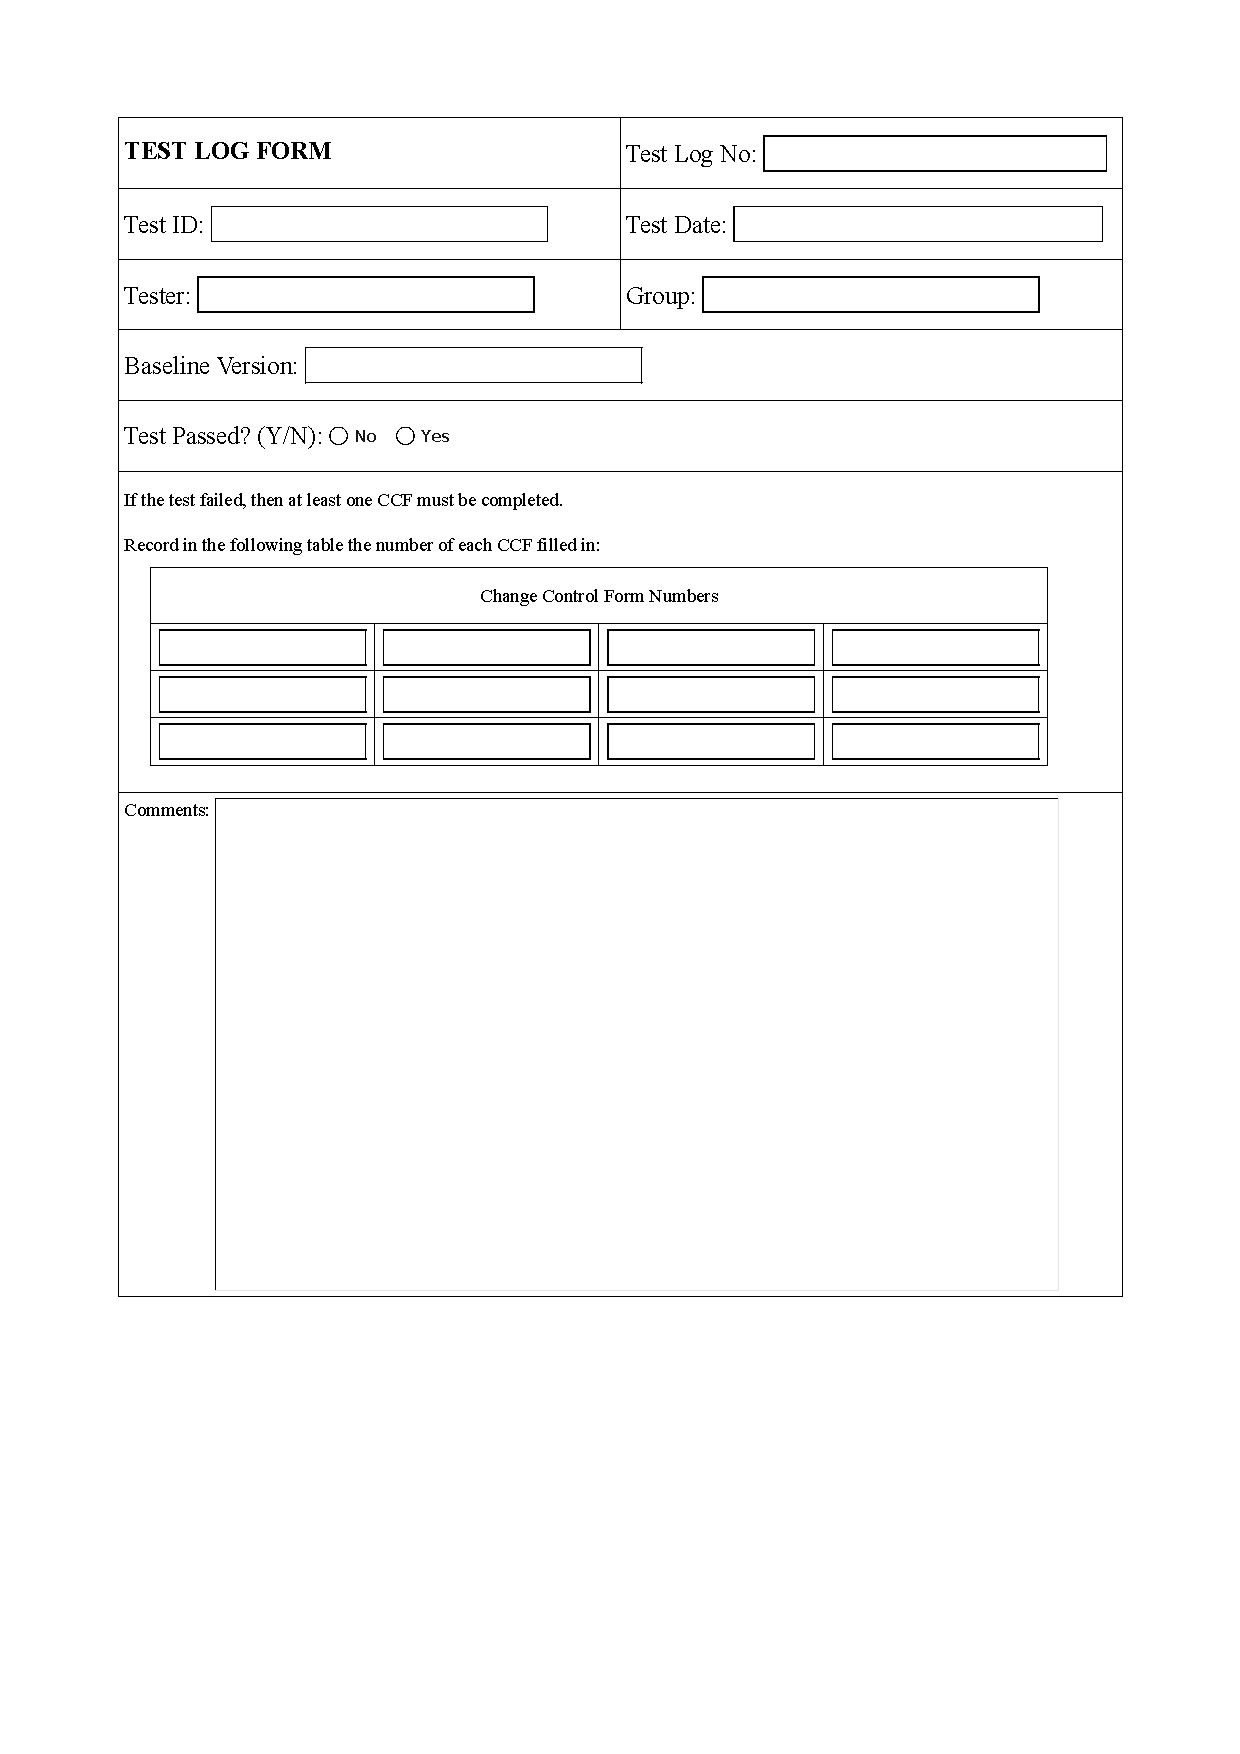
\includepdf{img/testlog.pdf}

\clearpage

\section{References}
\begin{thebibliography}{9}
\bibitem{Software Engineering Group Projects. QA Plan.} Software Engineering Group Projects. QA Plan. C. J. Price and N. W. Hardy. SE.QA.01. 1.8. Release.
\bibitem{Software Engineering Group Projects. Operating Procedures and Configuration Management Standards.} Software Engineering Group Projects. Operating Procedures and Configuration Management Standards.. C. J. Price and N.W Hardy. SE.QA.08. . 1.5. Release.
\bibitem{Software Engineering Group Projects. General Documentation Standards.}Software Engineering Group Projects. General Documentation Standards. C. J. Price and N. W. Hardy.
SE.QA.03. 1.5. Release.
\bibitem{Software Engineering Ian Sommerville Addison-Wesley Harlow}Software engineering Ian Sommerville Addison-Wesley Harlow; New York. 8th ed. ISBN: 0321313798
\bibitem{Software Engineering Group Projects. Producing A Final Report.}Software Engineering Group Projects. Producing A Final Report. C. J. Price. SE.QA.11. 1.4. Release.
\end{thebibliography}

\section{Document History}
\begin{tabular}{|l | l | l | l | l |}
\hline
Version & CCF No. & Date & Changes made to Document & Changed by \\
\hline
1.0 & N/A & 05/11/12 & Creation of first draft of document & CRH13\\
\hline
1.1 & N/A & 06/11/12 & Second draft, for review & CRH13\\
\hline
1.2 & 1,2,3 & 07/11/12 & Review & CRH13\\
\hline
1.3 & 4 & 11/11/12 & Spelling and grammatical errors & SIE5\\
\hline
1.4 & N/A & 12/11/12 & Ready for release & SIE5\\
\hline
\end{tabular}
\end{document}